\documentclass[12pt,a4paper]{article}\usepackage[]{graphicx}\usepackage[]{color}
% maxwidth is the original width if it is less than linewidth
% otherwise use linewidth (to make sure the graphics do not exceed the margin)
\makeatletter
\def\maxwidth{ %
  \ifdim\Gin@nat@width>\linewidth
    \linewidth
  \else
    \Gin@nat@width
  \fi
}
\makeatother

\definecolor{fgcolor}{rgb}{0.345, 0.345, 0.345}
\newcommand{\hlnum}[1]{\textcolor[rgb]{0.686,0.059,0.569}{#1}}%
\newcommand{\hlstr}[1]{\textcolor[rgb]{0.192,0.494,0.8}{#1}}%
\newcommand{\hlcom}[1]{\textcolor[rgb]{0.678,0.584,0.686}{\textit{#1}}}%
\newcommand{\hlopt}[1]{\textcolor[rgb]{0,0,0}{#1}}%
\newcommand{\hlstd}[1]{\textcolor[rgb]{0.345,0.345,0.345}{#1}}%
\newcommand{\hlkwa}[1]{\textcolor[rgb]{0.161,0.373,0.58}{\textbf{#1}}}%
\newcommand{\hlkwb}[1]{\textcolor[rgb]{0.69,0.353,0.396}{#1}}%
\newcommand{\hlkwc}[1]{\textcolor[rgb]{0.333,0.667,0.333}{#1}}%
\newcommand{\hlkwd}[1]{\textcolor[rgb]{0.737,0.353,0.396}{\textbf{#1}}}%
\let\hlipl\hlkwb

\usepackage{framed}
\makeatletter
\newenvironment{kframe}{%
 \def\at@end@of@kframe{}%
 \ifinner\ifhmode%
  \def\at@end@of@kframe{\end{minipage}}%
  \begin{minipage}{\columnwidth}%
 \fi\fi%
 \def\FrameCommand##1{\hskip\@totalleftmargin \hskip-\fboxsep
 \colorbox{shadecolor}{##1}\hskip-\fboxsep
     % There is no \\@totalrightmargin, so:
     \hskip-\linewidth \hskip-\@totalleftmargin \hskip\columnwidth}%
 \MakeFramed {\advance\hsize-\width
   \@totalleftmargin\z@ \linewidth\hsize
   \@setminipage}}%
 {\par\unskip\endMakeFramed%
 \at@end@of@kframe}
\makeatother

\definecolor{shadecolor}{rgb}{.97, .97, .97}
\definecolor{messagecolor}{rgb}{0, 0, 0}
\definecolor{warningcolor}{rgb}{1, 0, 1}
\definecolor{errorcolor}{rgb}{1, 0, 0}
\newenvironment{knitrout}{}{} % an empty environment to be redefined in TeX

\usepackage{alltt}
\usepackage[utf8]{inputenc}
\setlength{\paperheight}{11.7in} % set dimension of \paperwidth to 25 cm
\setlength{\paperwidth}{8.27in}
%%\addtolength{\paperheight}{2in} % enlarge \paperheight by 1 inch
\usepackage[portuguese]{babel}
\usepackage{longtable,booktabs}
\usepackage[T1]{fontenc}
\usepackage{a msmath}
\usepackage{indentfirst}
\usepackage{color}
\usepackage{caption}
\usepackage{amsfonts}
\usepackage{float}
\usepackage[dvipsnames]{xcolor}
\usepackage{amssymb}
\usepackage{graphicx}
\usepackage{lmodern}
\usepackage{subfigure}
\usepackage{caption}
\captionsetup{font=small}% \captionsetup{font=footnotesize}
\usepackage[left=1.5cm, right = 2cm, top=3cm,bottom=2.6cm]{geometry}
\fontsize{12pt}{10cm}\selectfont
\title{Análise descritiva e preditiva sobre \\ segmentação dos clientes Duas Rodas}
\usepackage{float}
\usepackage{fancyhdr}
%% SET DEFAULT FONTFD  
\usepackage{mathptmx}
\usepackage[T1]{fontenc}
%% \usepackage[T1]{fontenc}
%% \usepackage{times}
%% \usepackage{PTSerifCaption} 
%% \usepackage[T1]{fontenc}


\usepackage[T1]{fontenc}
\pagestyle{fancy}
\fancyhf{}
\fancyhead[LE,RO]{Mobills Labs}
\fancyhead[RE,LO]{{\small\scshape Relatório de Análise descritiva}}
\fancyfoot[CE,CO]{{\small\leftmark}}
\fancyfoot[LE,RO]{{\small\thepage}}

\renewcommand{\headrulewidth}{2pt}
\renewcommand{\footrulewidth}{1pt}
\IfFileExists{upquote.sty}{\usepackage{upquote}}{}
\begin{document}


\begin{titlepage}
\begin{center}
\begin{minipage}{5in}
\begin{center}
\hspace{-1cm}

\includegraphics[scale=0.23]{figure/logo.png}
\vspace{3.5cm}\\
{\large \scshape Relatório de Análise Descritiva}\\
\vspace{14cm}
{\hspace{1cm}
{\Large FORTALEZA \\ \hspace{1cm} 2018}}
\end{center}
\thispagestyle{empty}
\end{minipage}
\end{center}
\end{titlepage}

\newpage
\section{Análise das despesas}
A seguir temos o TOP 100 das Despesas que mais aparecem no dataset: 



\begin{knitrout}\small
\definecolor{shadecolor}{rgb}{0.969, 0.969, 0.969}\color{fgcolor}\begin{kframe}
\begin{verbatim}
##            used  (Mb) gc trigger  (Mb) max used  (Mb)
## Ncells  6621231 353.7   10018085 535.1  6621231 353.7
## Vcells 76979868 587.4  127031987 969.2 76979868 587.4
\end{verbatim}
\end{kframe}
\end{knitrout}
As medidas de resumo mostram que claramente há valores inválidos e outliers nos dados.

\begin{knitrout}\small
\definecolor{shadecolor}{rgb}{0.969, 0.969, 0.969}\color{fgcolor}\begin{kframe}


{\ttfamily\noindent\bfseries\color{errorcolor}{\#\# Error in cat(x, file = file, sep = c(rep.int(sep, ncolumns - 1), "{}\textbackslash{}n"{}), : objeto 'textoDesp' não encontrado}}\end{kframe}
\end{knitrout}
\begin{knitrout}\small
\definecolor{shadecolor}{rgb}{0.969, 0.969, 0.969}\color{fgcolor}\begin{kframe}
\begin{alltt}
\hlstd{Despesas} \hlopt
  \hlkwd{select}\hlstd{(ano,Valor)}\hlopt
  \hlkwd{split}\hlstd{(.}\hlopt{$}\hlstd{ano)} \hlopt
  \hlkwd{map}\hlstd{(summary)}
\end{alltt}
\begin{verbatim}
## $`2018`
##       ano           Valor        
##  Min.   :2018   Min.   : -10000  
##  1st Qu.:2018   1st Qu.:      9  
##  Median :2018   Median :     22  
##  Mean   :2018   Mean   :    133  
##  3rd Qu.:2018   3rd Qu.:     60  
##  Max.   :2018   Max.   :6000000  
## 
## $`2019`
##       ano           Valor                 
##  Min.   :2019   Min.   :          -15591  
##  1st Qu.:2019   1st Qu.:              10  
##  Median :2019   Median :              25  
##  Mean   :2019   Mean   :     12899026578  
##  3rd Qu.:2019   3rd Qu.:              69  
##  Max.   :2019   Max.   :9000000000000000
\end{verbatim}
\end{kframe}
\end{knitrout}
Para plotar o Histograma dos Valores gastos(Despesas) vamos limitar a variável `Valor` em até 1000 reais. Tendo em vista que quase a totalidade dos dadados se concentram nesse intervalo.
\begin{knitrout}\small
\definecolor{shadecolor}{rgb}{0.969, 0.969, 0.969}\color{fgcolor}\begin{kframe}
\begin{alltt}
\hlstd{Despesas} \hlopt
  \hlkwd{group_by}\hlstd{(UsuarioId,}
           \hlkwc{dia} \hlstd{= lubridate}\hlopt{::}\hlkwd{day}\hlstd{(DataDespesa),}
           \hlkwc{mes} \hlstd{= lubridate}\hlopt{::}\hlkwd{month}\hlstd{(DataDespesa),}
           \hlkwc{ano} \hlstd{= lubridate}\hlopt{::}\hlkwd{year}\hlstd{(DataDespesa))} \hlopt
    \hlkwd{summarise}\hlstd{(}\hlkwc{count} \hlstd{=} \hlkwd{n}\hlstd{(),} \hlkwc{valorSoma}\hlstd{=} \hlkwd{sum}\hlstd{(Valor))} \hlopt
    \hlkwd{arrange}\hlstd{(}\hlkwd{desc}\hlstd{(valorSoma))} \hlkwb{->} \hlstd{desp}



\hlstd{Despesas} \hlopt \hlstd{dplyr}\hlopt{::}\hlkwd{filter}\hlstd{(Valor} \hlopt{>} \hlnum{0} \hlopt{&} \hlstd{Valor} \hlopt{<} \hlnum{1000}\hlstd{)} \hlopt
    \hlkwd{ggplot}\hlstd{(}\hlkwd{aes}\hlstd{(Valor,}\hlkwc{y}\hlstd{=..density..))}\hlopt{+}
    \hlkwd{geom_histogram}\hlstd{(}\hlkwc{fill}\hlstd{=}\hlstr{"white"}\hlstd{,}\hlkwc{alpha}\hlstd{=}\hlnum{0.8}\hlstd{)}\hlopt{+}
    \hlkwd{facet_grid}\hlstd{(}\hlopt{~}\hlstd{ano )}\hlopt{+}\hlstd{temaMobills}\hlopt{+}
        \hlkwd{labs}\hlstd{(}\hlkwc{title}\hlstd{=}\hlstr{"Distribuição das despesas"}\hlstd{)}\hlopt{+}
    \hlkwd{scale_x_continuous}\hlstd{(}\hlkwc{limits}\hlstd{=}\hlkwd{c}\hlstd{(}\hlnum{0}\hlstd{,}\hlnum{1000}\hlstd{))}
\end{alltt}
\end{kframe}
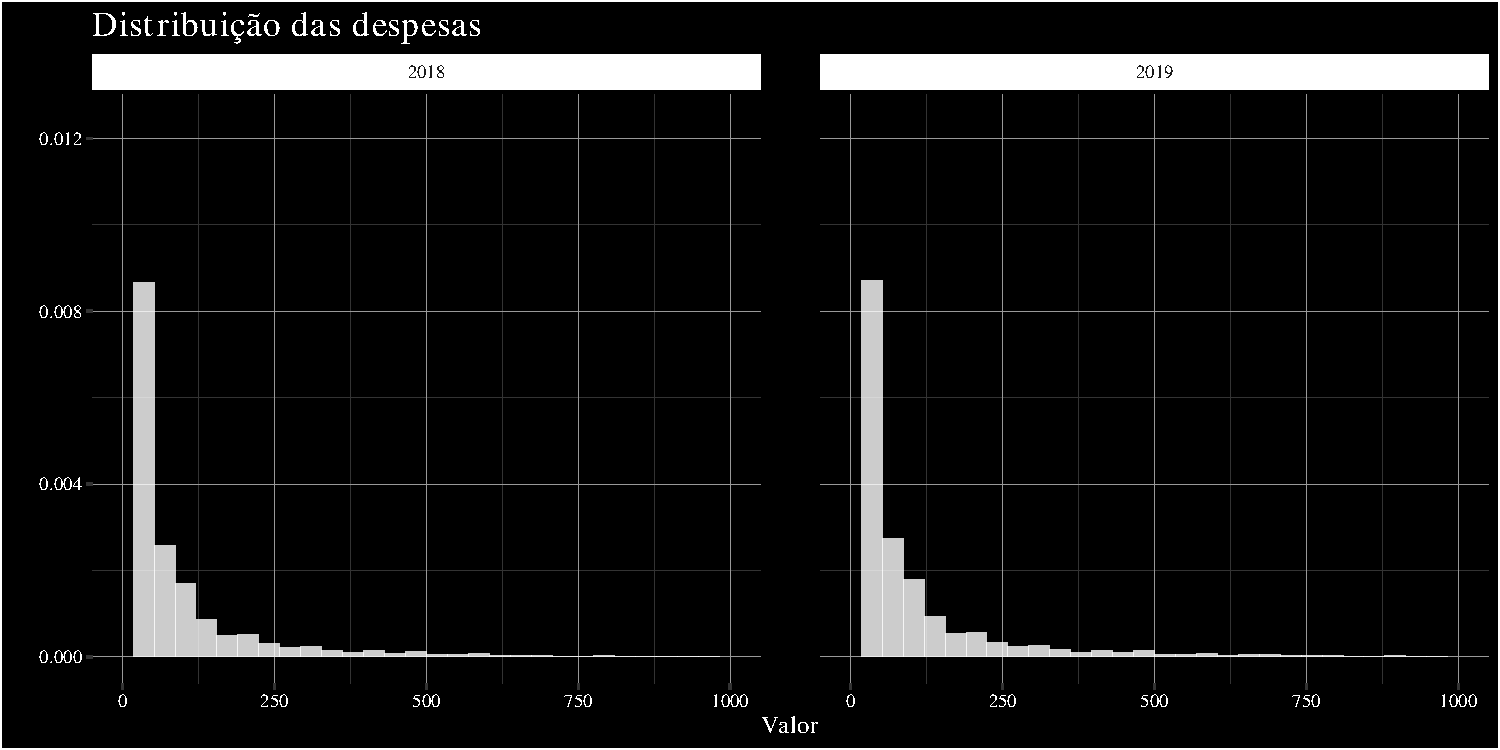
\includegraphics[width=\maxwidth]{figure/unnamed-chunk-5-1} 
\begin{kframe}\begin{alltt}
\hlcom{##histogram by month}
\hlstd{Despesas} \hlopt \hlstd{dplyr}\hlopt{::}\hlkwd{filter}\hlstd{(Valor} \hlopt{>} \hlnum{0} \hlopt{&} \hlstd{Valor} \hlopt{<} \hlnum{1000}\hlstd{)} \hlopt
    \hlkwd{ggplot}\hlstd{(}\hlkwd{aes}\hlstd{(Valor,}\hlkwc{y}\hlstd{=..density..))}\hlopt{+}
    \hlkwd{geom_histogram}\hlstd{(}\hlkwc{fill}\hlstd{=}\hlstr{"white"}\hlstd{,}\hlkwc{alpha}\hlstd{=}\hlnum{0.8}\hlstd{)}\hlopt{+}
    \hlkwd{facet_grid}\hlstd{(}\hlopt{~}\hlstd{ano )}\hlopt{+}\hlstd{temaMobills}\hlopt{+}
        \hlkwd{labs}\hlstd{(}\hlkwc{title}\hlstd{=}\hlstr{"Distribuição das despesas"}\hlstd{)}\hlopt{+}
    \hlkwd{scale_x_continuous}\hlstd{(}\hlkwc{limits}\hlstd{=}\hlkwd{c}\hlstd{(}\hlnum{0}\hlstd{,}\hlnum{1000}\hlstd{))}\hlopt{+}
  \hlkwd{facet_wrap}\hlstd{(}\hlopt{~}\hlstd{mes)}
\end{alltt}
\end{kframe}
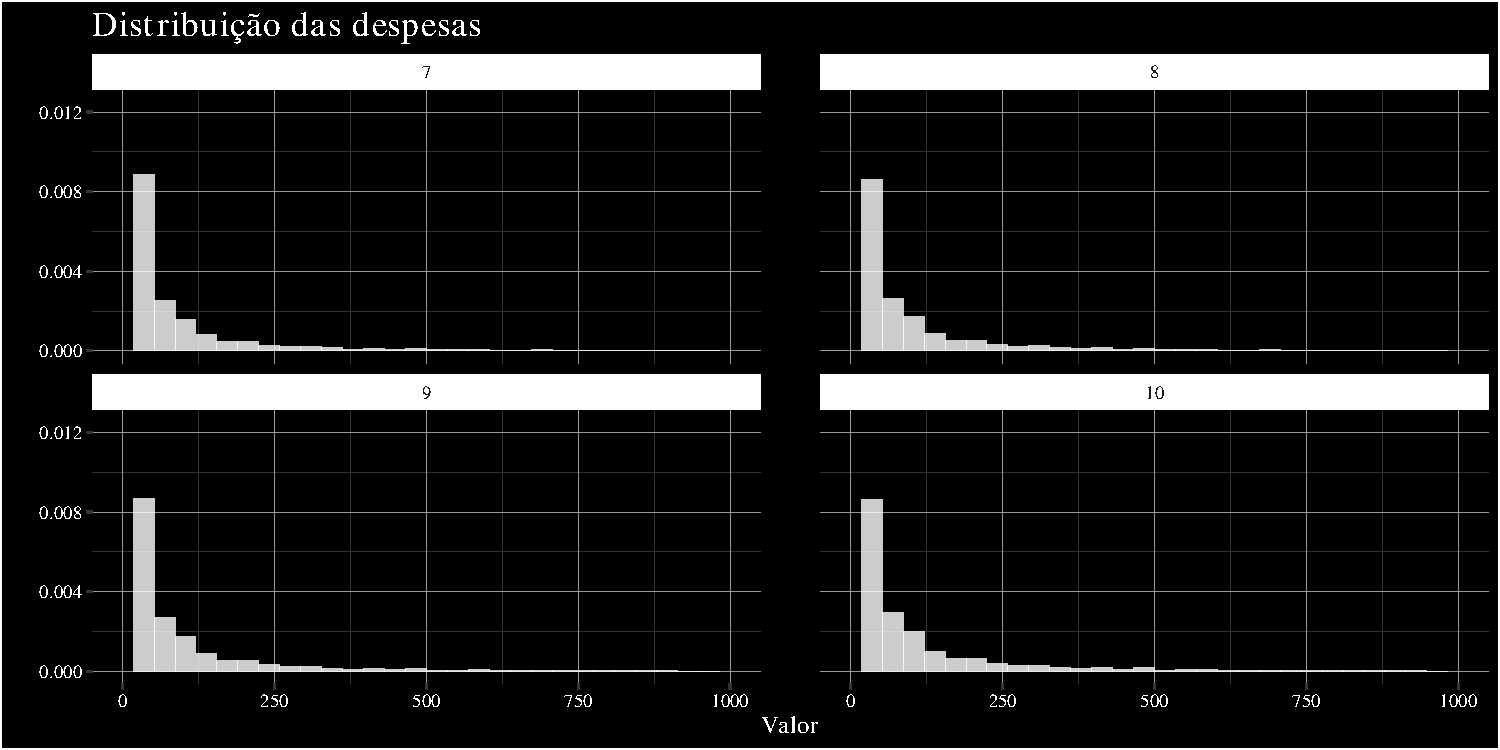
\includegraphics[width=\maxwidth]{figure/unnamed-chunk-5-2} 

\end{knitrout}


\begin{knitrout}\small
\definecolor{shadecolor}{rgb}{0.969, 0.969, 0.969}\color{fgcolor}\begin{kframe}
\begin{alltt}
\hlstd{desp} \hlopt
  \hlkwd{group_by}\hlstd{(mes,ano)} \hlopt
  \hlkwd{summarise}\hlstd{(}\hlkwc{contagem}\hlstd{=}\hlkwd{n}\hlstd{())} \hlopt
  \hlkwd{ggplot}\hlstd{(}\hlkwd{aes}\hlstd{(mes, contagem,}\hlkwc{labs}\hlstd{=contagem))}\hlopt{+}
  \hlkwd{geom_col}\hlstd{(}\hlkwd{aes}\hlstd{(}\hlkwc{fill}\hlstd{=contagem),}
           \hlkwc{width} \hlstd{=} \hlnum{0.5}\hlstd{)}\hlopt{+}
  \hlkwd{scale_fill_viridis}\hlstd{(}\hlkwc{option}\hlstd{=}\hlstr{"magma"}\hlstd{,}\hlkwc{begin}\hlstd{=}\hlnum{0.5}\hlstd{)}\hlopt{+}
  \hlkwd{labs}\hlstd{(}\hlkwc{title}\hlstd{=}\hlstr{"Quantidade de Despesas por mês"}\hlstd{,}
       \hlkwc{subtitle} \hlstd{=} \hlstr{"Usuarios de 16 à 24 anos, no periodo de 11 de Julho à 10 de Outubro."}\hlstd{,}
       \hlkwc{x}\hlstd{=}\hlstr{"Mês"}\hlstd{,}
       \hlkwc{y}\hlstd{=}\hlstr{"Quantidade de despesas"}\hlstd{)}\hlopt{+}
  \hlstd{temaMobills}\hlopt{+}
  \hlkwd{scale_y_continuous}\hlstd{(}\hlkwc{limits} \hlstd{=} \hlkwd{c}\hlstd{(}\hlnum{0}\hlstd{,}\hlnum{100000}\hlstd{),}
                       \hlkwc{expand}\hlstd{=}\hlkwd{c}\hlstd{(}\hlnum{0.01009}\hlstd{,}\hlnum{0.000000001}\hlstd{),}
                       \hlkwc{breaks} \hlstd{=} \hlkwd{seq}\hlstd{(}\hlnum{0}\hlstd{,}\hlnum{150000}\hlstd{,}\hlnum{10000}\hlstd{))}\hlopt{+}
  \hlkwd{geom_text}\hlstd{(}\hlkwd{aes}\hlstd{(}\hlkwc{label}\hlstd{=contagem),}
              \hlkwc{size}\hlstd{=}\hlnum{3.5}\hlstd{,}
              \hlkwc{colour}\hlstd{=}\hlstr{"white"}\hlstd{,}
              \hlkwc{vjust}\hlstd{=}\hlopt{-}\hlnum{0.2}\hlstd{)}\hlopt{+}
  \hlkwd{facet_grid}\hlstd{(}\hlopt{~}\hlstd{ano)}
\end{alltt}
\end{kframe}
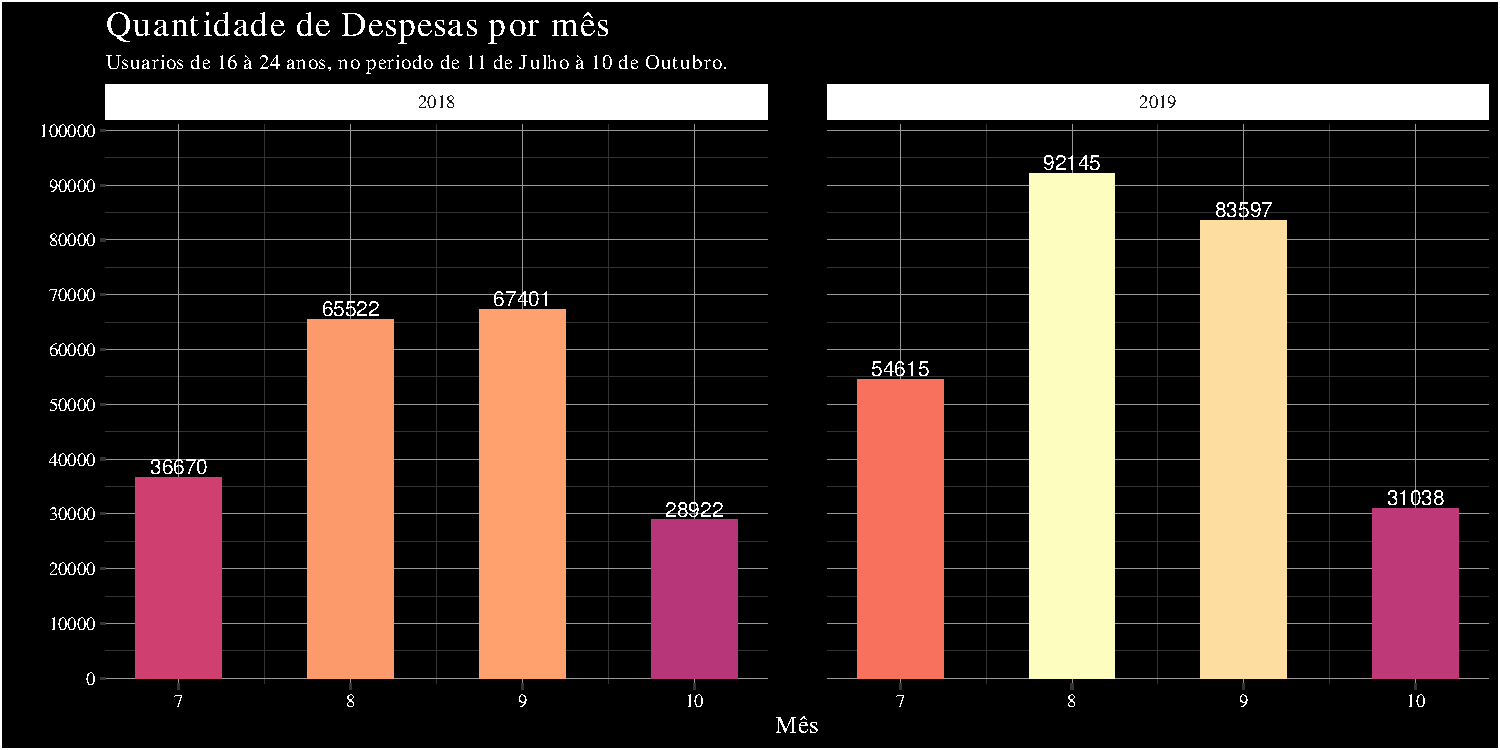
\includegraphics[width=\maxwidth]{figure/unnamed-chunk-6-1} 

\end{knitrout}


\begin{knitrout}\small
\definecolor{shadecolor}{rgb}{0.969, 0.969, 0.969}\color{fgcolor}\begin{kframe}
\begin{alltt}
\hlstd{Despesas} \hlopt
    \hlkwd{group_by}\hlstd{(Descricao)} \hlopt
    \hlkwd{summarise}\hlstd{(}\hlkwc{count} \hlstd{=} \hlkwd{n}\hlstd{(),} \hlkwc{valorSoma}\hlstd{=} \hlkwd{sum}\hlstd{(Valor))} \hlopt
    \hlkwd{top_n}\hlstd{(}\hlnum{100000}\hlstd{)} \hlopt \hlkwd{filter}\hlstd{(count} \hlopt{>} \hlnum{3000}\hlstd{)} \hlopt \hlkwd{arrange}\hlstd{(}\hlkwd{desc}\hlstd{(count))}\hlopt
  \hlkwd{ggplot}\hlstd{(}\hlkwd{aes}\hlstd{(}\hlkwc{x}\hlstd{=}\hlkwd{reorder}\hlstd{(Descricao,count,max),count),}\hlkwc{labels}\hlstd{=count)}\hlopt{+}
  \hlkwd{geom_col}\hlstd{(}\hlkwc{fill}\hlstd{=}\hlstr{"white"}\hlstd{,}\hlkwc{width} \hlstd{=} \hlnum{0.5}\hlstd{)}\hlopt{+}
  \hlkwd{coord_flip}\hlstd{()}\hlopt{+}
  \hlstd{temaMobills}\hlopt{+}
  \hlkwd{theme}\hlstd{(}\hlkwc{axis.text} \hlstd{=} \hlkwd{element_text}\hlstd{(}\hlkwc{size}\hlstd{=}\hlnum{7}\hlstd{),}
        \hlkwc{panel.grid.major.x} \hlstd{=}\hlkwd{element_line}\hlstd{(}\hlkwc{colour}\hlstd{=}\hlstr{"white"}\hlstd{,}\hlkwc{linetype} \hlstd{=} \hlnum{1}\hlstd{),}
        \hlkwc{panel.grid.minor.x} \hlstd{=} \hlkwd{element_blank}\hlstd{(),}
        \hlkwc{panel.grid.major.y} \hlstd{=} \hlkwd{element_line}\hlstd{(}\hlkwc{size}\hlstd{=}\hlnum{0.1}\hlstd{))}\hlopt{+}
  \hlkwd{geom_text}\hlstd{(}\hlkwd{aes}\hlstd{(}\hlkwc{label}\hlstd{=count),}\hlkwc{colour}\hlstd{=}\hlstr{"white"}\hlstd{,}\hlkwc{size}\hlstd{=}\hlnum{3}\hlstd{,}\hlkwc{hjust}\hlstd{=}\hlopt{-}\hlnum{0.5}\hlstd{)}\hlopt{+}
  \hlkwd{scale_y_continuous}\hlstd{(}\hlkwc{limits}\hlstd{=}\hlkwd{c}\hlstd{(}\hlnum{0}\hlstd{,}\hlnum{32000}\hlstd{))}
\end{alltt}
\end{kframe}
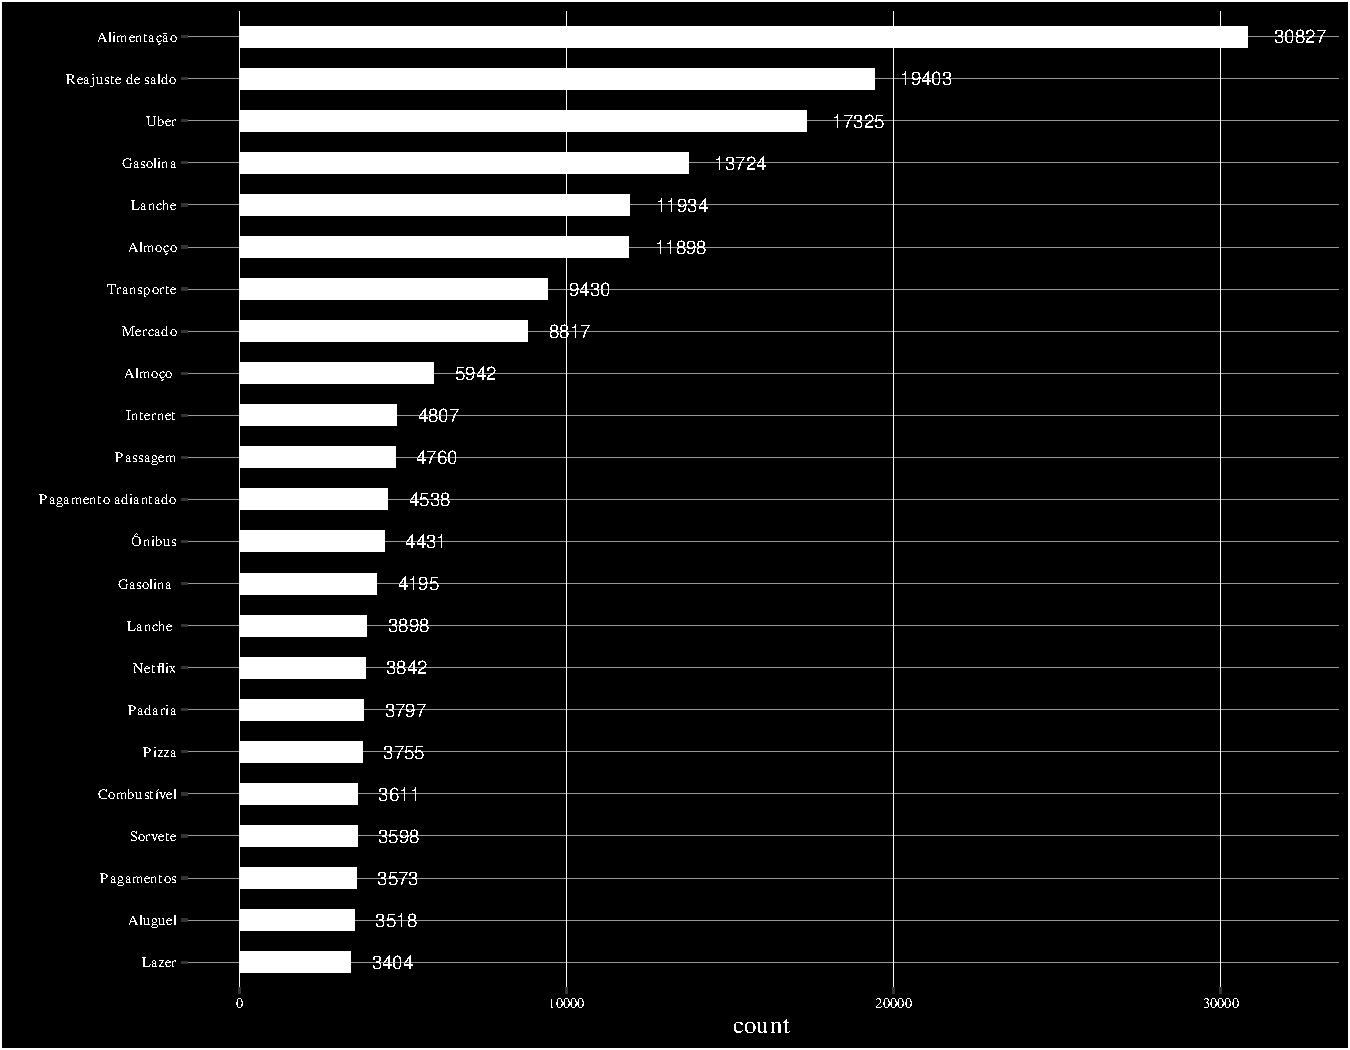
\includegraphics[width=\maxwidth]{figure/unnamed-chunk-7-1} 

\end{knitrout}



\begin{knitrout}\small
\definecolor{shadecolor}{rgb}{0.969, 0.969, 0.969}\color{fgcolor}\begin{kframe}
\begin{alltt}
\hlstd{Despesas} \hlopt
    \hlkwd{group_by}\hlstd{(Descricao)} \hlopt
    \hlkwd{summarise}\hlstd{(}\hlkwc{count} \hlstd{=} \hlkwd{n}\hlstd{(),} \hlkwc{valorSoma}\hlstd{=} \hlkwd{sum}\hlstd{(Valor))} \hlopt
    \hlkwd{top_n}\hlstd{(}\hlnum{100000}\hlstd{)} \hlopt \hlkwd{filter}\hlstd{(count} \hlopt{<}\hlnum{3000}\hlstd{,count}\hlopt{>}\hlnum{1500}\hlstd{)} \hlopt
  \hlkwd{arrange}\hlstd{(}\hlkwd{desc}\hlstd{(count))}\hlopt
  \hlkwd{ggplot}\hlstd{(}\hlkwd{aes}\hlstd{(}\hlkwc{x}\hlstd{=}\hlkwd{reorder}\hlstd{(Descricao,count,max),count),}\hlkwc{labels} \hlstd{= count)}\hlopt{+}
  \hlkwd{geom_col}\hlstd{(}\hlkwc{fill}\hlstd{=}\hlstr{"white"}\hlstd{,}\hlkwc{width} \hlstd{=} \hlnum{0.5}\hlstd{)}\hlopt{+}
  \hlkwd{coord_flip}\hlstd{()}\hlopt{+}
  \hlstd{temaMobills}\hlopt{+}
  \hlkwd{theme}\hlstd{(}\hlkwc{axis.text} \hlstd{=} \hlkwd{element_text}\hlstd{(}\hlkwc{size}\hlstd{=}\hlnum{7}\hlstd{),}
        \hlkwc{panel.grid.major.x} \hlstd{=}\hlkwd{element_line}\hlstd{(}\hlkwc{colour}\hlstd{=}\hlstr{"white"}\hlstd{,}\hlkwc{linetype} \hlstd{=} \hlnum{1}\hlstd{),}
        \hlkwc{panel.grid.minor.x} \hlstd{=} \hlkwd{element_blank}\hlstd{(),}
        \hlkwc{panel.grid.major.y} \hlstd{=} \hlkwd{element_line}\hlstd{(}\hlkwc{size}\hlstd{=}\hlnum{0.1}\hlstd{))}\hlopt{+}
  \hlkwd{geom_text}\hlstd{(}\hlkwd{aes}\hlstd{(}\hlkwc{label}\hlstd{=count),}\hlkwc{colour}\hlstd{=}\hlstr{"white"}\hlstd{,}\hlkwc{size}\hlstd{=}\hlnum{3}\hlstd{,}\hlkwc{hjust}\hlstd{=}\hlopt{-}\hlnum{0.5}\hlstd{)}\hlopt{+}
  \hlkwd{scale_y_continuous}\hlstd{(}\hlkwc{limits}\hlstd{=}\hlkwd{c}\hlstd{(}\hlnum{0}\hlstd{,}\hlnum{32000}\hlstd{))}
\end{alltt}
\end{kframe}
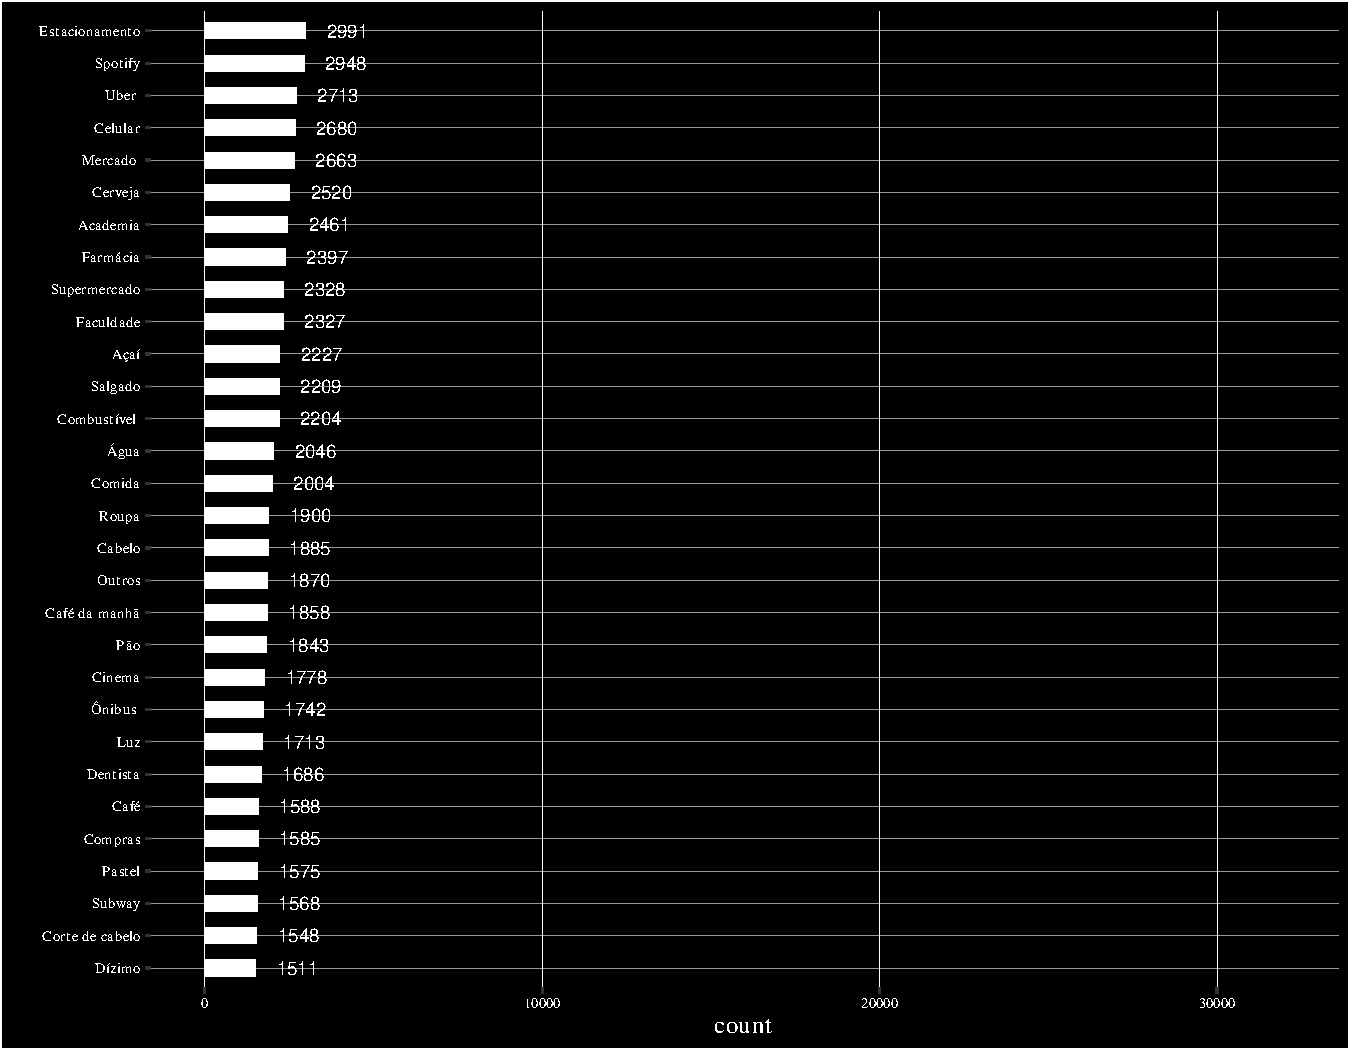
\includegraphics[width=\maxwidth]{figure/unnamed-chunk-8-1} 

\end{knitrout}

Qual o tipo  de despesa com o maior gasto total?

\begin{knitrout}\small
\definecolor{shadecolor}{rgb}{0.969, 0.969, 0.969}\color{fgcolor}\begin{kframe}
\begin{alltt}
\hlstd{Despesas} \hlopt
    \hlstd{dplyr}\hlopt{::}\hlkwd{filter}\hlstd{(Valor} \hlopt{>} \hlnum{0} \hlopt{&} \hlstd{Valor} \hlopt{<} \hlnum{2000}\hlstd{)} \hlopt
    \hlkwd{group_by}\hlstd{(Descricao)} \hlopt
    \hlkwd{summarise}\hlstd{(}\hlkwc{count} \hlstd{=} \hlkwd{n}\hlstd{(),} \hlkwc{valorSoma}\hlstd{=} \hlkwd{sum}\hlstd{(Valor))} \hlopt
    \hlkwd{arrange}\hlstd{(}\hlkwd{desc}\hlstd{(valorSoma))} \hlopt \hlkwd{top_n}\hlstd{(}\hlnum{20}\hlstd{)}
\end{alltt}
\begin{verbatim}
## # A tibble: 20 x 3
##    Descricao           count valorSoma
##    <chr>               <int>     <dbl>
##  1 Reajuste de saldo   19122  2043250.
##  2 Aluguel              3471  1735572.
##  3 Alimentação         30777  1058510.
##  4 Faculdade            2313   793314.
##  5 Gasolina            13724   659972.
##  6 Pagamento adiantado  2389   626031.
##  7 Carro                1369   618208.
##  8 Pagamentos           3542   543463.
##  9 "Aluguel "            994   465695.
## 10 Mercado              8786   411919.
## 11 Celular              2670   396889.
## 12 Internet             4804   376046.
## 13 Nubank               1012   341527.
## 14 Moradia              1389   331761.
## 15 "Faculdade "          834   274922.
## 16 Transporte           9393   270631.
## 17 Uber                17317   261770.
## 18 Moto                  974   239474.
## 19 Empréstimo            911   231605.
## 20 Almoço              11898   225157.
\end{verbatim}
\end{kframe}
\end{knitrout}



Agora iremos agrupar as depesas por categoria

\begin{knitrout}\small
\definecolor{shadecolor}{rgb}{0.969, 0.969, 0.969}\color{fgcolor}\begin{kframe}
\begin{alltt}
\hlstd{DespesasCat} \hlkwb{<-} \hlkwd{mutate}\hlstd{(DespesasCat,}
                      \hlkwc{chave} \hlstd{=} \hlkwd{paste0}\hlstd{(DespesasCat}\hlopt{$}\hlstd{Id,DespesasCat}\hlopt{$}\hlstd{UsuarioId))}
\hlstd{Despesas} \hlkwb{<-} \hlkwd{mutate}\hlstd{(Despesas,}
                      \hlkwc{chave} \hlstd{=} \hlkwd{paste0}\hlstd{(Despesas}\hlopt{$}\hlstd{TipoDespesaId,Despesas}\hlopt{$}\hlstd{UsuarioId))}
\hlstd{Despesas2} \hlkwb{<-} \hlkwd{left_join}\hlstd{(Despesas,DespesasCat,}\hlkwc{by}\hlstd{=}\hlkwd{c}\hlstd{(}\hlstr{'chave'} \hlstd{=} \hlstr{'chave'}\hlstd{))}

\hlstd{Despesas2} \hlopt \hlkwd{mutate}\hlstd{(}\hlkwc{chaveUnica} \hlstd{=} \hlkwd{paste0}\hlstd{(Descricao, Nome, UsuarioId.x),}
                     \hlkwc{dia} \hlstd{= lubridate}\hlopt{::}\hlkwd{day}\hlstd{(Despesas2}\hlopt{$}\hlstd{DataDespesa),}
                     \hlkwc{mes} \hlstd{= lubridate}\hlopt{::}\hlkwd{month}\hlstd{(Despesas2}\hlopt{$}\hlstd{DataDespesa),}
                     \hlkwc{ano} \hlstd{= lubridate}\hlopt{::}\hlkwd{year}\hlstd{(Despesas2}\hlopt{$}\hlstd{DataDespesa))} \hlkwb{->} \hlstd{Despesas2}

\hlcom{##Despesas2 %>% select(Descricao,}
\hlcom{##Nome,}
\hlcom{##TipoDespesaId,}
\hlcom{##UsuarioId.x,}
\hlcom{##UsuarioId.y,}
\hlcom{##chaveUnica,}
\hlcom{##mes) %>% }
\hlcom{##distinct() %>% View()}
\hlcom{##Despesas2[unique(Despesas2$chaveUnica), ] }
\hlcom{##Despesas2[duplicated(Despesas2$chaveUnica), ]%>% View}
\hlcom{##length(Despesas2$chaveUnica)}


\hlcom{##Despesas2 %>% group_by(Descricao,Nome,mes) %>% }
\hlcom{##summarise(contagem= n()) %>%}
\hlcom{##top_n(100) %>% View()}
\end{alltt}
\end{kframe}
\end{knitrout}

\begin{knitrout}\small
\definecolor{shadecolor}{rgb}{0.969, 0.969, 0.969}\color{fgcolor}\begin{kframe}
\begin{alltt}
\hlstd{text} \hlkwb{<-} \hlkwd{readLines}\hlstd{(}\hlstr{"./texto.txt"}\hlstd{)}
\hlstd{docs} \hlkwb{<-} \hlkwd{Corpus}\hlstd{(}\hlkwd{VectorSource}\hlstd{(text))}
\hlstd{docs} \hlkwb{<-} \hlkwd{tm_map}\hlstd{(docs, toSpace,} \hlstr{"/"}\hlstd{)}
\hlstd{docs} \hlkwb{<-} \hlkwd{tm_map}\hlstd{(docs, toSpace,} \hlstr{"@"}\hlstd{)}
\hlstd{docs} \hlkwb{<-} \hlkwd{tm_map}\hlstd{(docs, toSpace,} \hlstr{"\textbackslash{}\textbackslash{}|"}\hlstd{)}
\hlstd{tm_ma}
\end{alltt}


{\ttfamily\noindent\bfseries\color{errorcolor}{\#\# Error in eval(expr, envir, enclos): objeto 'tm\_ma' não encontrado}}\begin{alltt}
\hlstd{docs} \hlkwb{<-} \hlkwd{tm_map}\hlstd{(docs,} \hlkwd{content_transformer}\hlstd{(tolower))}
\hlcom{# Remove numbers}
\hlstd{docs} \hlkwb{<-} \hlkwd{tm_map}\hlstd{(docs, removeNumbers)}
\hlcom{# Remove english common stopwords}
\hlstd{docs} \hlkwb{<-} \hlkwd{tm_map}\hlstd{(docs, removeWords,} \hlkwd{stopwords}\hlstd{(}\hlstr{"portuguese"}\hlstd{))}
\hlcom{# Remove your own stop word}
\hlcom{# specify your stopwords as a character vector}
\hlstd{docs} \hlkwb{<-} \hlkwd{tm_map}\hlstd{(docs, removeWords,} \hlkwd{c}\hlstd{(}\hlstr{"blabla1"}\hlstd{,} \hlstr{"blabla2"}\hlstd{))}
\hlcom{# Remove punctuations}
\hlstd{docs} \hlkwb{<-} \hlkwd{tm_map}\hlstd{(docs, removePunctuation)}
\hlcom{# Eliminate extra white spaces}
\hlstd{docs} \hlkwb{<-} \hlkwd{tm_map}\hlstd{(docs, stripWhitespace)}
\hlcom{# Text stemming}
\hlcom{# docs <- tm_map(docs, stemDocument)}

\hlstd{dtm} \hlkwb{<-} \hlkwd{TermDocumentMatrix}\hlstd{(docs)}
\hlstd{m} \hlkwb{<-} \hlkwd{as.matrix}\hlstd{(dtm)}
\hlstd{v} \hlkwb{<-} \hlkwd{sort}\hlstd{(}\hlkwd{rowSums}\hlstd{(m),}\hlkwc{decreasing}\hlstd{=}\hlnum{TRUE}\hlstd{)}
\hlstd{d} \hlkwb{<-} \hlkwd{data.frame}\hlstd{(}\hlkwc{word} \hlstd{=} \hlkwd{names}\hlstd{(v),}\hlkwc{freq}\hlstd{=v)}
\hlkwd{head}\hlstd{(d,}\hlnum{20}\hlstd{)}
\end{alltt}
\begin{verbatim}
##                    word   freq
## alimentação alimentação 322355
## transporte   transporte 123890
## pagamentos   pagamentos  99637
## lazer             lazer  69323
## moradia         moradia  39244
## saúde             saúde  35075
## roupa             roupa  32306
## educação       educação  26014
## outros           outros  25733
## reajuste       reajuste  22964
## cartão           cartão  12876
## compras         compras  11744
## despesas       despesas  10086
## mercado         mercado  10069
## crédito         crédito   9873
## carro             carro   9846
## casa               casa   9595
## gastos           gastos   9481
## beleza           beleza   8631
## presente       presente   7593
\end{verbatim}
\begin{alltt}
\hlkwd{set.seed}\hlstd{(}\hlnum{1234}\hlstd{)}
\hlkwd{wordcloud}\hlstd{(}\hlkwc{words} \hlstd{= d}\hlopt{$}\hlstd{word,} \hlkwc{freq} \hlstd{= d}\hlopt{$}\hlstd{freq,}\hlkwc{scale}\hlstd{=}\hlkwd{c}\hlstd{(}\hlnum{3}\hlstd{,}\hlnum{0.6}\hlstd{),} \hlkwc{min.freq} \hlstd{=} \hlnum{500}\hlstd{,}
          \hlkwc{max.words}\hlstd{=}\hlnum{200}\hlstd{,} \hlkwc{random.order}\hlstd{=}\hlnum{FALSE}\hlstd{,} \hlkwc{rot.per}\hlstd{=}\hlnum{0.35}\hlstd{,}
          \hlkwc{colors}\hlstd{=}\hlkwd{brewer.pal}\hlstd{(}\hlnum{8}\hlstd{,} \hlstr{"Dark2"}\hlstd{))}
\end{alltt}
\end{kframe}
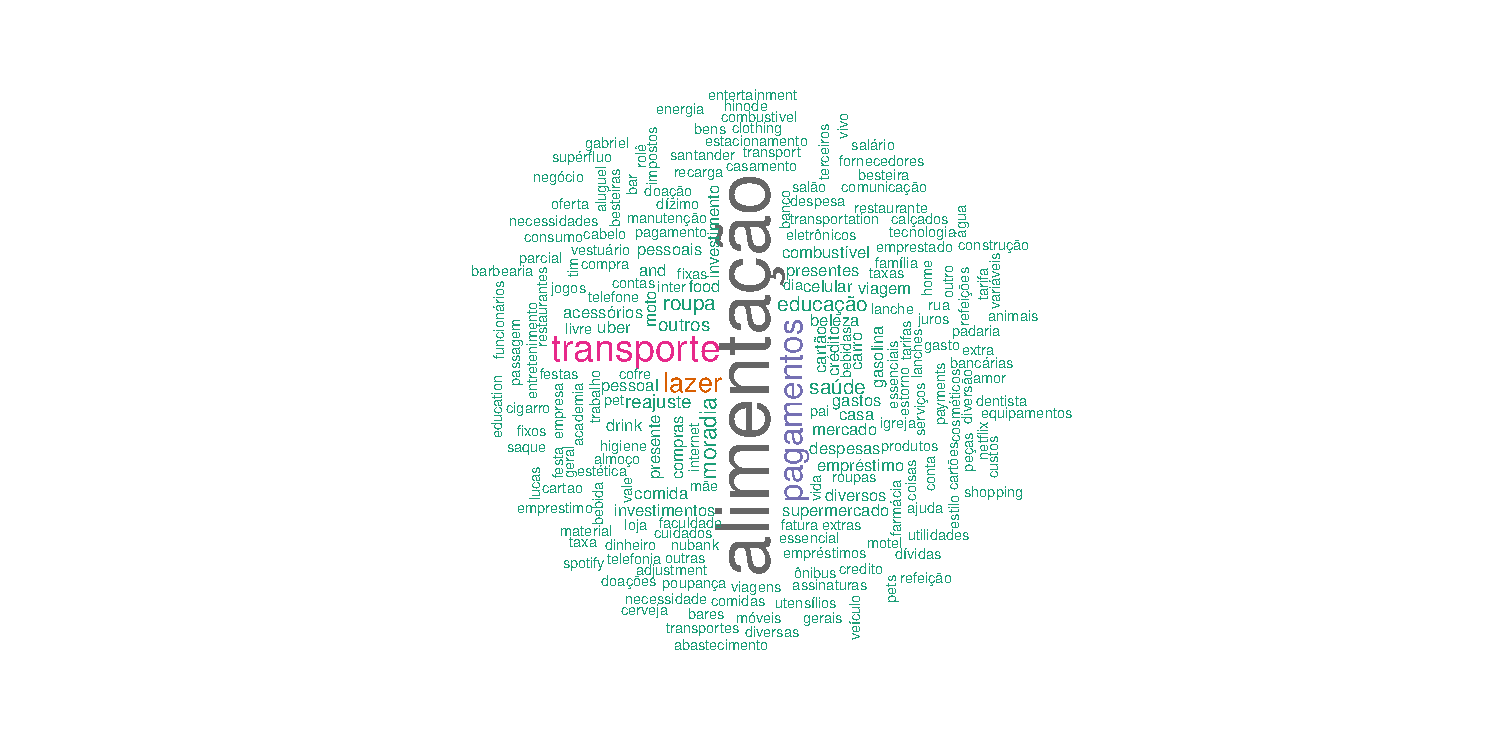
\includegraphics[width=\maxwidth]{figure/unnamed-chunk-11-1} 

\end{knitrout}

\begin{knitrout}\small
\definecolor{shadecolor}{rgb}{0.969, 0.969, 0.969}\color{fgcolor}\begin{kframe}
\begin{alltt}
\hlcom{# Build Dataset}

\hlstd{Despesas2} \hlopt \hlkwd{select}\hlstd{(Nome,Descricao)} \hlopt
  \hlkwd{group_by}\hlstd{(Nome,Descricao)} \hlopt
  \hlkwd{summarise}\hlstd{(}\hlkwc{count}\hlstd{=}\hlkwd{n}\hlstd{())} \hlopt \hlkwd{arrange}\hlstd{(}\hlkwd{desc}\hlstd{(count))} \hlopt \hlkwd{top_n}\hlstd{(}\hlnum{50}\hlstd{)} \hlopt \hlkwd{head}\hlstd{(}\hlnum{100}\hlstd{)} \hlopt
  \hlkwd{treemap}\hlstd{(}\hlkwc{index}\hlstd{=}\hlkwd{c}\hlstd{(}\hlstr{"Nome"}\hlstd{,}\hlstr{"Descricao"}\hlstd{),}
            \hlkwc{vSize}\hlstd{=}\hlstr{"count"}\hlstd{,}
            \hlkwc{vColor} \hlstd{=} \hlstr{"Nome"}\hlstd{,}
            \hlkwc{type}\hlstd{=}\hlstr{"index"}\hlstd{,}\hlkwc{range}\hlstd{=}\hlkwd{c}\hlstd{(}\hlnum{0}\hlstd{,}\hlnum{10000}\hlstd{)}
            \hlstd{)}
\end{alltt}
\end{kframe}
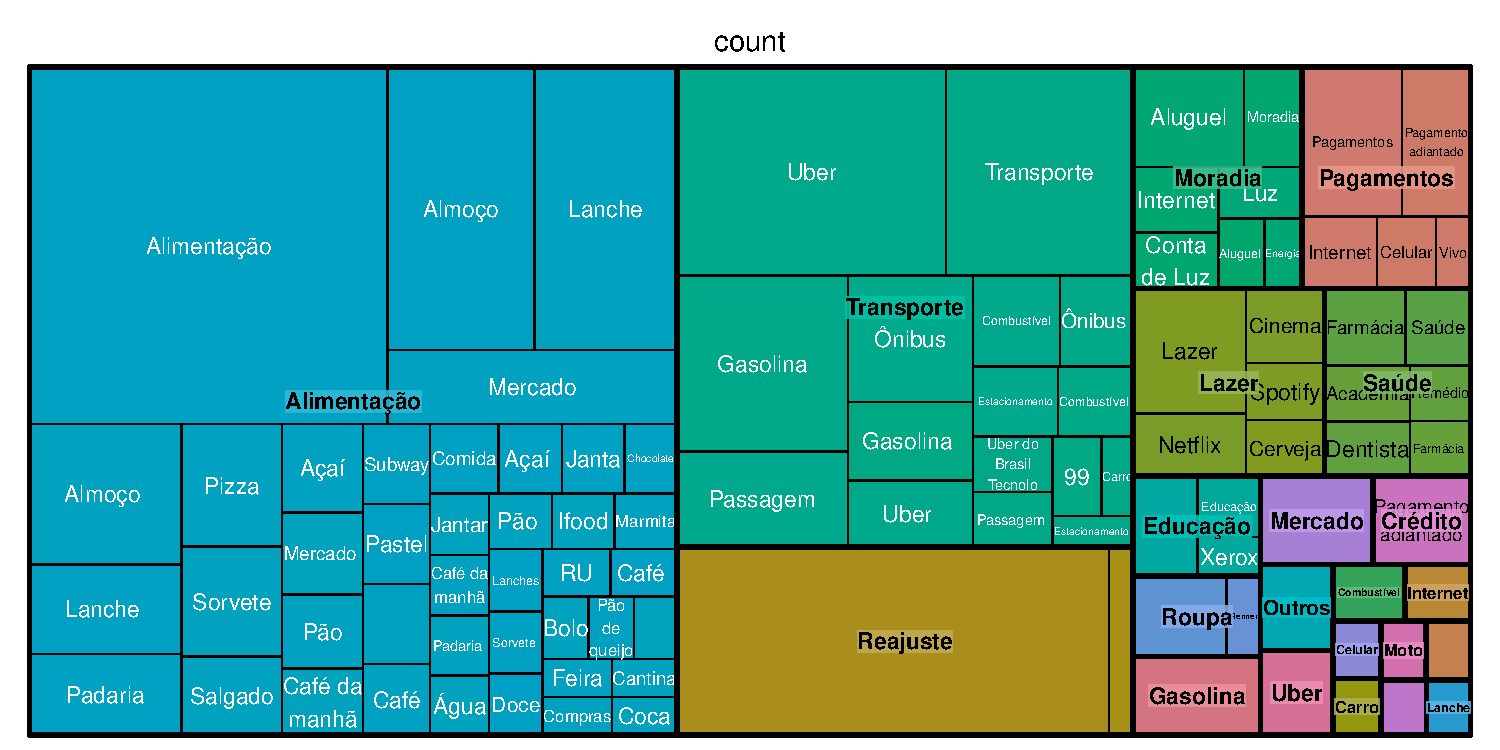
\includegraphics[width=\maxwidth]{figure/unnamed-chunk-12-1} 

\end{knitrout}
\section{Análise das Receitas}



\begin{knitrout}\small
\definecolor{shadecolor}{rgb}{0.969, 0.969, 0.969}\color{fgcolor}
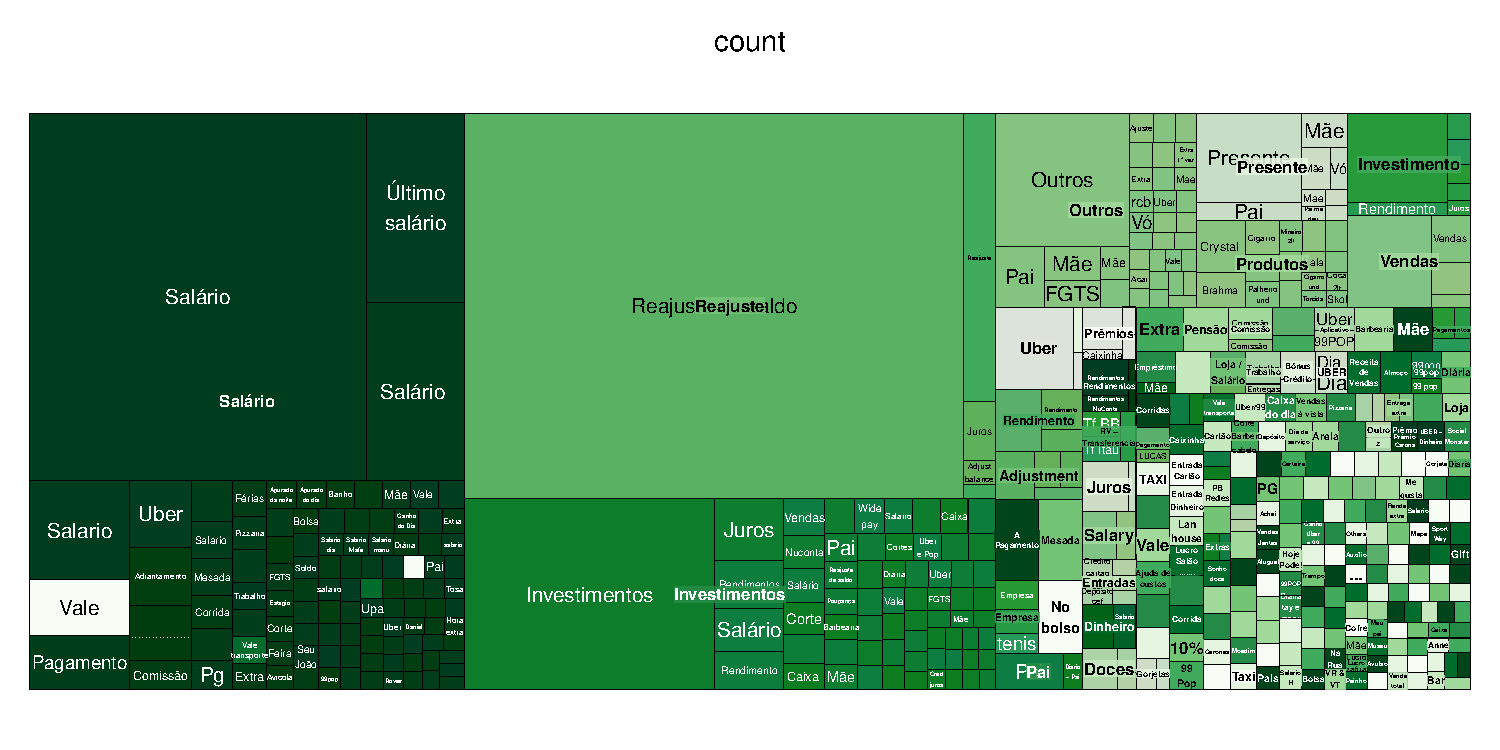
\includegraphics[width=\maxwidth]{figure/unnamed-chunk-14-1} 

\end{knitrout}

\begin{knitrout}\small
\definecolor{shadecolor}{rgb}{0.969, 0.969, 0.969}\color{fgcolor}\begin{kframe}
\begin{alltt}
\hlstd{textr} \hlkwb{<-} \hlkwd{readLines}\hlstd{(}\hlstr{"./textoReceitas.txt"}\hlstd{)}
\hlstd{docsr} \hlkwb{<-} \hlkwd{Corpus}\hlstd{(}\hlkwd{VectorSource}\hlstd{(textr))}
\hlstd{docsr} \hlkwb{<-} \hlkwd{tm_map}\hlstd{(docsr, toSpace,} \hlstr{"/"}\hlstd{)}
\hlstd{docsr} \hlkwb{<-} \hlkwd{tm_map}\hlstd{(docsr, toSpace,} \hlstr{"@"}\hlstd{)}
\hlstd{docsr} \hlkwb{<-} \hlkwd{tm_map}\hlstd{(docsr, toSpace,} \hlstr{"\textbackslash{}\textbackslash{}|"}\hlstd{)}

\hlstd{docsr} \hlkwb{<-} \hlkwd{tm_map}\hlstd{(docsr,} \hlkwd{content_transformer}\hlstd{(tolower))}
\hlcom{# Remove numbers}
\hlstd{docsr} \hlkwb{<-} \hlkwd{tm_map}\hlstd{(docsr, removeNumbers)}
\hlcom{# Remove english common stopwords}
\hlstd{docsr} \hlkwb{<-} \hlkwd{tm_map}\hlstd{(docsr, removeWords,} \hlkwd{stopwords}\hlstd{(}\hlstr{"portuguese"}\hlstd{))}
\hlcom{# Remove your own stop word}
\hlcom{# specify your stopwords as a character vector}
\hlcom{##docsr <- tm_map(docsr, removeWords, c("blabla1", "blabla2")) }
\hlcom{# Remove punctuations}
\hlstd{docsr} \hlkwb{<-} \hlkwd{tm_map}\hlstd{(docsr, removePunctuation)}
\hlcom{# Eliminate extra white spaces}
\hlstd{docsr} \hlkwb{<-} \hlkwd{tm_map}\hlstd{(docsr, stripWhitespace)}
\hlcom{# Text stemming}
\hlcom{# docs <- tm_map(docs, stemDocument)}

\hlstd{dtmr} \hlkwb{<-} \hlkwd{TermDocumentMatrix}\hlstd{(docsr)}
\hlstd{mr} \hlkwb{<-} \hlkwd{as.matrix}\hlstd{(dtmr)}
\hlstd{vr} \hlkwb{<-} \hlkwd{sort}\hlstd{(}\hlkwd{rowSums}\hlstd{(mr),}\hlkwc{decreasing}\hlstd{=}\hlnum{TRUE}\hlstd{)}
\hlstd{dr} \hlkwb{<-} \hlkwd{data.frame}\hlstd{(}\hlkwc{word} \hlstd{=} \hlkwd{names}\hlstd{(vr),}\hlkwc{freq}\hlstd{=vr)}
\hlkwd{head}\hlstd{(dr,}\hlnum{10}\hlstd{)}
\end{alltt}
\begin{verbatim}
##                        word  freq
## salário             salário 61896
## investimentos investimentos 33263
## reajuste           reajuste 28335
## outros               outros 27834
## presente           presente  6928
## vendas               vendas  6553
## investimento   investimento  5618
## empréstimo       empréstimo  4036
## cartão               cartão  3767
## pagamento         pagamento  3480
\end{verbatim}
\begin{alltt}
\hlkwd{set.seed}\hlstd{(}\hlnum{1234}\hlstd{)}
\hlkwd{wordcloud}\hlstd{(}\hlkwc{words} \hlstd{= dr}\hlopt{$}\hlstd{word,} \hlkwc{freq} \hlstd{= dr}\hlopt{$}\hlstd{freq,}\hlkwc{scale}\hlstd{=}\hlkwd{c}\hlstd{(}\hlnum{3}\hlstd{,}\hlnum{0.4}\hlstd{),} \hlkwc{min.freq} \hlstd{=} \hlnum{200}\hlstd{,}
          \hlkwc{max.words}\hlstd{=}\hlnum{200}\hlstd{,} \hlkwc{random.order}\hlstd{=}\hlnum{FALSE}\hlstd{,} \hlkwc{rot.per}\hlstd{=}\hlnum{0.35}\hlstd{,}
          \hlkwc{colors}\hlstd{=}\hlkwd{brewer.pal}\hlstd{(}\hlnum{8}\hlstd{,} \hlstr{"Dark2"}\hlstd{))}
\end{alltt}
\end{kframe}
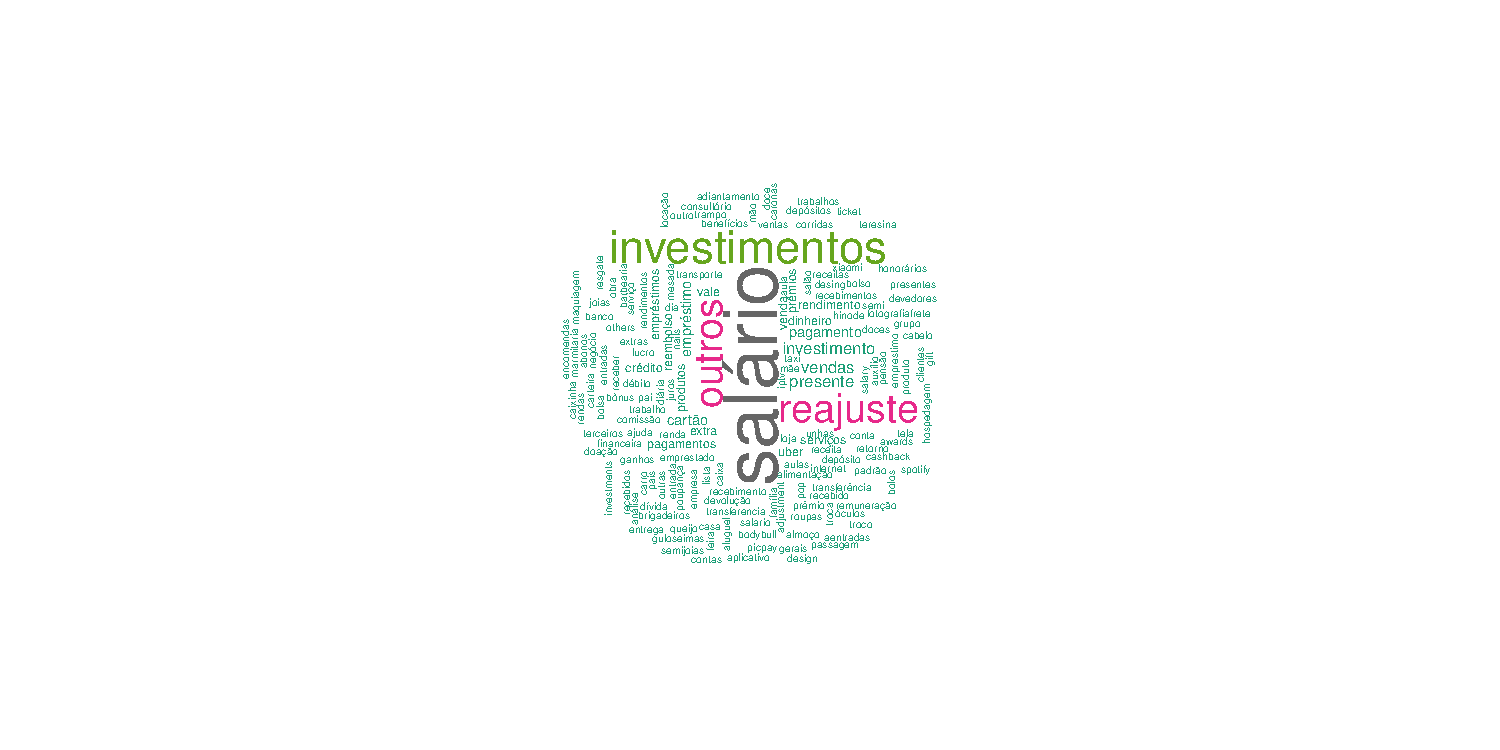
\includegraphics[width=\maxwidth]{figure/cloundReceitas-1} 

\end{knitrout}

\end{document}


